\documentclass{sigplanconf}

\usepackage{ifthen}
\usepackage{fancyvrb}
\usepackage{color}
\usepackage{ulem}
\usepackage{xspace}
\usepackage{relsize}
\usepackage{epsfig}
\usepackage{amssymb}
\usepackage{amsmath}
\usepackage{amsfonts}
\usepackage[utf8]{inputenc}
\usepackage{setspace}

\usepackage{listings}

\usepackage[T1]{fontenc}
\usepackage[scaled=0.8]{beramono}


\definecolor{commentgray}{rgb}{0.3,0.3,0.3}

\lstset{
  basicstyle=\ttfamily\footnotesize,
  language=Python,
  keywordstyle=\bfseries,
  stringstyle=\color{blue},
  commentstyle=\color{commentgray}\textit,
  fancyvrb=true,
  showstringspaces=false,
  %keywords={def,while,if,elif,return,class,get,set,new,guard_class}
  numberstyle = \tiny,
  numbersep = -20pt,
}

\newboolean{showcomments}
\setboolean{showcomments}{false}
\ifthenelse{\boolean{showcomments}}
  {\newcommand{\nb}[2]{
    \fbox{\bfseries\sffamily\scriptsize#1}
    {\sf\small$\blacktriangleright$\textit{#2}$\blacktriangleleft$}
   }
   \newcommand{\version}{\emph{\scriptsize$-$Id: main.tex 19055 2008-06-05 11:20:31Z cfbolz $-$}}
  }
  {\newcommand{\nb}[2]{}
   \newcommand{\version}{}
  }

\newcommand\cfbolz[1]{\nb{CFB}{#1}}
\newcommand\toon[1]{\nb{TOON}{#1}}
\newcommand\anto[1]{\nb{ANTO}{#1}}
\newcommand\arigo[1]{\nb{AR}{#1}}
\newcommand\fijal[1]{\nb{FIJAL}{#1}}
\newcommand\pedronis[1]{\nb{PEDRONIS}{#1}}
\newcommand{\commentout}[1]{}

\newcommand\ie{i.e.,\xspace}
\newcommand\eg{e.g.,\xspace}

\normalem

\let\oldcite=\cite

\renewcommand\cite[1]{\ifthenelse{\equal{#1}{XXX}}{[citation~needed]}{\oldcite{#1}}}

% compressing itemize env, in case we need it
\newenvironment{zitemize}% zero - line spacing itemize environment
   {\begin{list}{--}{
   \setlength{\itemsep}{0 pt}
   \setlength{\parsep}{0 pt}
   \setlength{\topsep} {0 pt} }}% the end stuff
   {\end{list}}

\definecolor{gray}{rgb}{0.5,0.5,0.5}

\begin{document}

\title{Runtime Feedback in a Meta-Tracing JIT for Efficient Dynamic Languages}

\authorinfo{Carl Friedrich Bolz$^a$ \and Antonio Cuni$^a$ \and Maciej Fijałkowski$^b$ \and Michael Leuschel$^a$ \and \\
            Samuele Pedroni$^c$ \and Armin Rigo$^a$}
           {$^a$Heinrich-Heine-Universität Düsseldorf, STUPS Group, Germany

            $^b$merlinux GmbH, Hildesheim, Germany

            $^c$Open End, Göteborg, Sweden
           }
           {cfbolz@gmx.de \and anto.cuni@gmail.com \and fijal@merlinux.eu \and
           leuschel@cs.uni-duesseldorf.de \and samuele.pedroni@gmail.com \and arigo@tunes.org}

\conferenceinfo{ICOOOLPS}{'11 Lancaster, UK}
\CopyrightYear{2011}
\crdata{XXX}

\maketitle

\category{D.3.4}{Programming Languages}{Processors}[code generation,
incremental compilers, interpreters, run-time environments]

\begin{abstract}

Meta-tracing JITs can be applied to a variety of different
languages without explicitly encoding language semantics into the compiler. So
far, they lacked a way to feed back runtime information into the
compiler, which restricted their performance. In this paper we describe the
flexible mechanisms in PyPy's meta-tracing JIT that can be used to control runtime feedback in language-specific ways. These mechanisms are flexible
enough to implement classical VM techniques such as maps and polymorphic inline
caches.

\end{abstract}


%___________________________________________________________________________
\section{Introduction}

One of the hardest parts of implementing a dynamic language efficiently is to
optimize its object model. This is made harder by the fact that many recent
languages such as Python, JavaScript or Ruby have rather complex core object
semantics. For them, even implementing just an interpreter is already a complex
task. Implementing them efficiently with a just-in-time compiler (JIT) is
extremely challenging, because of their many corner-cases.

It has long been an objective of the partial evaluation community to
automatically produce compilers from interpreters. There has been a
renaissance of this idea around the approach of tracing just-in-time
compilers. A number of projects have attempted this approach. SPUR \cite{bebenita_spur:_2010} is
a tracing JIT for .NET together with a JavaScript implementation in C\#. PyPy
\cite{armin_rigo_pypys_2006} contains a tracing JIT for RPython \cite{davide_ancona_rpython:_2007} (a restricted
subset of Python). This JIT is then used to trace a number of languages
implementations written in RPython. A number of other experiments in this
directions were done, such as an interpreter for Lua in JavaScript, which is run
on and optimized with a tracing JIT for JavaScript
\cite{yermolovich_optimization_2009}.

These projects have in common that they work one meta-level down, providing a tracing JIT for the
language used to implement the dynamic language, and not for the dynamic language itself.
The tracing JIT will then trace through the object model of the dynamic
language implementation. This makes the object model transparent to the tracer
and its optimizations. Therefore the semantics of the dynamic language does not
have to be replicated in a JIT. We call this approach \emph{meta-tracing}.
Another commonality of these approaches is that they allow some annotations (or
hints) in the dynamic language implementation to guide the meta-tracer. This
makes the process not completely automatic but can give good speedups over
bare meta-tracing.

In this paper we present two of these hints that are extensively used in the
PyPy project to improve the performance of its Python interpreter. 

Conceptually, the significant speed-ups that can be achieved with
dynamic compilation depend on feeding into compilation and exploiting
values observed at runtime. In particular, if
there are values which vary very slowly, it is possible to compile multiple
specialized versions of the same code, one for each actual value.  To exploit
the runtime feedback, the implementation code and data structures need to be
structured so that many such slow-varying values are at hand. The hints that
we present precisely allow us to implement such feedback and exploitation in a
meta-tracing context.

Concretely these hints are used to control how the optimizer of the
tracing JIT can improve the traces of the object model. In particular the hints
influence the constant folding
optimization. The first hint makes it possible to turn arbitrary
variables in the trace into constant by feeding back runtime values. The
second hint allows the definition of additional foldable operations.

Together these two hints can be used to express many classic implementation
techniques used for object models of dynamic languages, such as maps and
polymorphic inline caches.

The contributions of this paper are:
\begin{itemize}
 \item A hint to turn arbitrary variables into constants in the trace, that
 means the feedback of runtime information into compilation.
 \item A way to define new pure operations which the constant folding
 optimization then recognizes.
 \item A worked-out example of a simple object model of a dynamic language and
 how it can be improved using these hints.
\end{itemize}

The paper is structured as follows: Section~\ref{sec:Background} gives an
introduction to the PyPy project and meta-tracing and presents an example of a
tiny dynamic language object model. Section~\ref{sec:hints} presents the hints,
what they do and how they are applied. Section~\ref{sec:fastobjmodel} shows how
the hints are applied to the tiny object model and Section~\ref{sec:evaluation}
presents benchmarks.

\cfbolz{XXX stress more that "the crux of the techniques and a significant
portion of new contributions in the paper are from how to refactoring codes to
expose likely runtime constants and pure functions"}


\section{Background}
\label{sec:Background}

\subsection{The PyPy Project}
\label{sub:pypy}

The PyPy project \cite{armin_rigo_pypys_2006} strives to be an environment where
complex dynamic languages can be implemented efficiently. The approach taken
when implementing a language with PyPy is to write an interpreter for the language
in \emph{RPython}. RPython is a restricted subset of Python chosen in such a way
that it is possible to perform type inference on it. The interpreters in RPython
can therefore be translated to efficient C code.

A number of languages have been implemented with PyPy, most importantly a full
Python implementation, but also a Prolog interpreter
\cite{carl_friedrich_bolz_towards_2010} and a Smalltalk VM
\cite{carl_friedrich_bolz_back_2008}.

The translation of the interpreter to C code adds a number of implementation details into the
final executable that are not present in the interpreter implementation, such as
a garbage collector. The interpreter can therefore be kept free from low-level
implementation details. Another aspect of the final VM that is added
semi-automatically to the generated VM is a tracing JIT compiler.

The advantage of this approach is that writing an interpreter is much easier
and less error prone than manually writing a JIT compiler.  Similarly, writing
in a high level language such as RPython is easier than writing in C.

We call the code that runs on top of an interpreter implemented with PyPy the
\emph{user code} or \emph{user program}.

%___________________________________________________________________________
\subsection{PyPy's Meta-Tracing JIT Compilers}
\label{sub:tracing}

A recently popular approach to JIT compilers is that of tracing JITs. Tracing
JITs have their origin in the Dynamo project, which used one of them for dynamic
assembler optimization \cite{bala_dynamo:_2000}. Later they were used to implement
a lightweight JIT for Java \cite{gal_hotpathvm:_2006} and for dynamic languages such as
JavaScript \cite{gal_trace-based_2009}.

A tracing JIT works by recording traces of concrete execution paths through the
program. Those
traces are therefore linear list of operations, which are optimized and then
get turned into machine code. This recording automatically inlines functions:
when a function call is encountered the operations of the called functions are
simply put into the trace of the caller too. The tracing JIT tries to produce traces
that correspond to loops in the traced program, but most tracing JITs now also
have support for tracing non-loops \cite{andreas_gal_incremental_2006}.

Because the traces always correspond to a concrete execution they cannot
contain any control flow splits. Therefore they encode the control flow
decisions needed to stay on the trace with the help of \emph{guards}. Those are
operations that check that the assumptions are still true when the compiled trace is later executed with different values.

To be able to do this recording, VMs with a
tracing JIT typically contain an interpreter. After a user program is
started the interpreter is used; only the most frequently executed paths through the user
program are turned into machine code. The interpreter is also used when a guard
fails to continue the execution from the failing guard.

One disadvantage of (tracing) JITs which makes them not directly applicable to
PyPy is that they need to encode the language semantics of the language they are
tracing. Since PyPy wants to be a
general framework, we want to reuse our tracer for different languages.
Therefore PyPy's JIT is a \emph{meta-tracer} \cite{bolz_tracing_2009}. It does not
trace the execution of the user program, but instead traces the execution of
the \emph{interpreter} that is running the program. This means that the traces
it produces don't contain the bytecodes of the language in question, but
RPython-level operations that the interpreter did to execute the program.

Tracing through the execution of an interpreter has many advantages. It makes
the tracer, its optimizers and backends reusable for a variety of languages. The
language semantics do not need to be encoded into the JIT. Instead the tracer
just picks them up from the interpreter. This also means that the JIT by
construction supports the full language.

While the operations in a trace are those of the interpreter, the loops that are
traced by the tracer are the loops in the
user program. To achieve this the tracer stops tracing after one iteration of
the loop in the user function that is being considered. At this point, it probably
traced many iterations of the interpreter main loop.

\begin{figure}
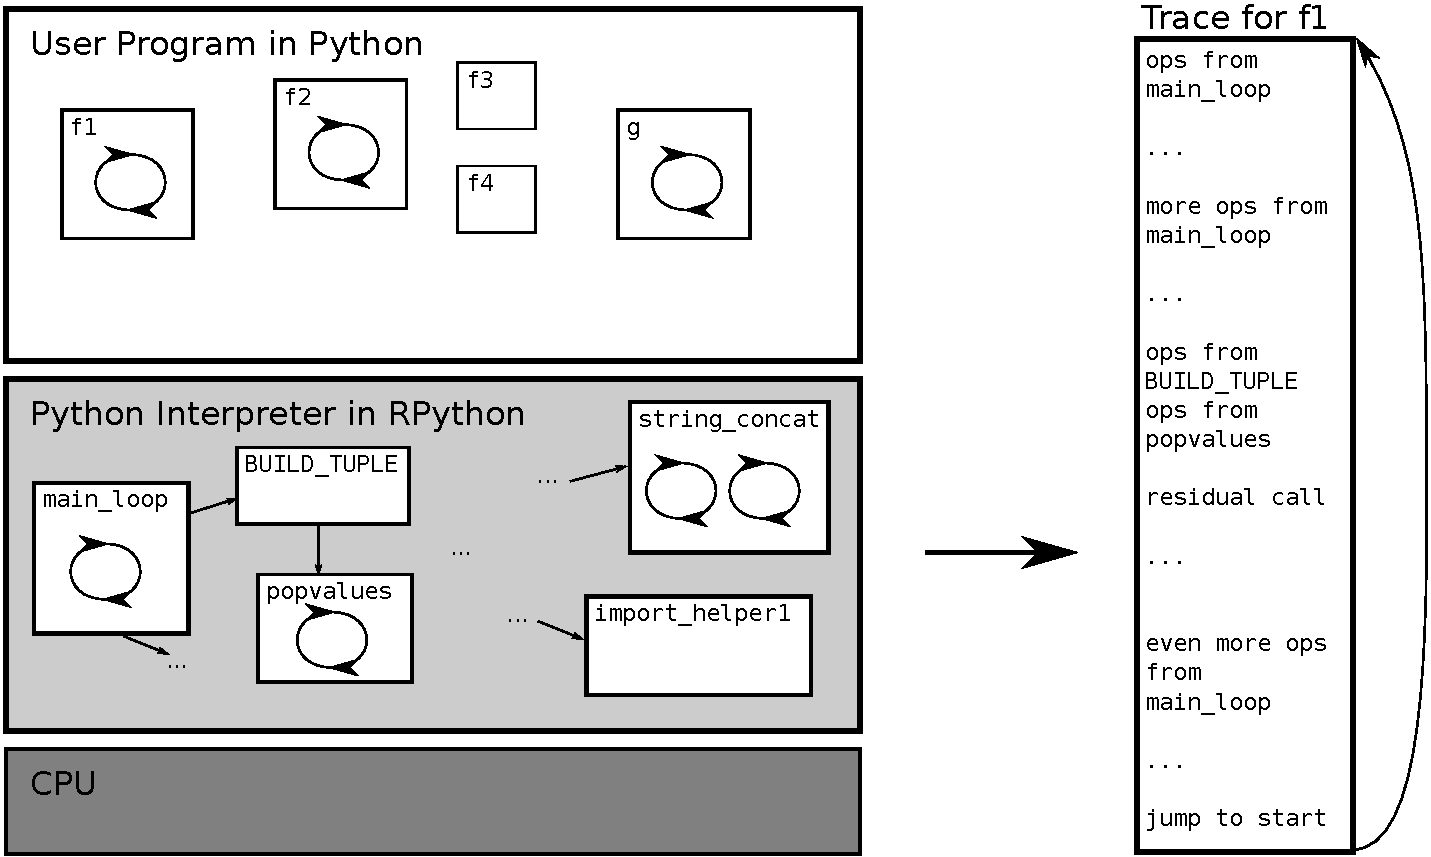
\includegraphics[scale=0.5]{figures/trace-levels}
\caption{The levels involved in tracing}
\label{fig:trace-levels}
\end{figure}

Figure~\ref{fig:trace-levels} shows a diagram of the process. On the left are
the levels of execution. The CPU executes the binary of
PyPy's Python interpreter, which consists of RPython functions that have been
compiled first to C, then to machine code. The interpreter runs a Python program written by a
programmer (the user). If the tracer is used, it traces operations on the level
of the interpreter. However, the extent of the trace is determined by the loops
in the user program.


\subsection{Optimizing Traces}
\label{sub:optimizing}

Before sending the trace to the backend to produce actual machine code, it is
optimized.  The optimizer applies a number of techniques to remove or simplify
the operations in the trace. Most of these are well known compiler optimization
techniques, with the difference that it is easier to apply them in a tracing
JIT because it only has to deal with linear traces.  Among the techniques are
constant folding, common subexpression elimination, allocation removal
\cite{bolz_allocation_2011}, store/load propagation, loop invariant code
motion.

In some places it turns out that if the interpreter author rewrites some parts
of the interpreter with these optimizations in mind the traces that are produced
by the optimizer can be vastly improved.

\subsection{Running Example}
\label{sub:running}
\anto{this example is not referenced until section \ref{sec:fastobjmodel}: I
  would put it just before it}

As the running example of this paper we will use a very simple and bare-bones
object model that just supports classes and instances, without any
inheritance or other advanced features. The model has classes, which contain methods.
Instances have a class. Instances have their own attributes (or fields). When looking up an
attribute on an instance, the instances attributes are searched. If the
attribute is not found there, the class' methods are searched.

\begin{figure}
\begin{lstlisting}[mathescape,basicstyle=\ttfamily,numbers = right]
class Class(object):
    def __init__(self, name):
        self.name = name
        self.methods = {}

    def instantiate(self):
        return Instance(self)

    def find_method(self, name):
        return self.methods.get(name, None)

    def write_method(self, name, value):
        self.methods[name] = value


class Instance(object):
    def __init__(self, cls):
        self.cls = cls
        self.attributes = {}

    def getfield(self, name):
        return self.attributes.get(name, None)

    def write_attribute(self, name, value):
        self.attributes[name] = value

    def getattr(self, name):
	result = self.getfield(name)
	if result is None:
            result = self.cls.find_method(name)
	    if result is None:
		raise AttributeError
	return result
\end{lstlisting}

\caption{Original Version of a Simple Object Model}
\label{fig:interpreter-slow}
\end{figure}


To implement this object model, we could use the RPython code in
Figure~\ref{fig:interpreter-slow} as part of the interpreter source code.
In this straightforward implementation the methods and attributes are just
stored in dictionaries (hash maps) on the classes and instances, respectively.
While this object model is very
simple it already contains most hard parts of Python's object model. Both
instances and classes can have arbitrary fields, and they are changeable at
any time.  Moreover, instances can change their class after they have been
created.

When using this object model in
an interpreter, a huge amount of time will be spent doing lookups in these
dictionaries.
Let's assume we trace through code that sums three attributes, such as:
\anto{I still think it's a bit weird to call them ``methods'' and then use
  them as attributes in the example}

\begin{lstlisting}[mathescape,basicstyle=\ttfamily]
inst.getattr("a") + inst.getattr("b") + inst.getattr("c")
\end{lstlisting}

\begin{figure}
\begin{Verbatim}
# inst.getattr("a")
attributes1 = inst.attributes
result1 = dict.get(attributes1, "a")
guard(result1 is not None)

# inst.getattr("b")
attributes2 = inst.attributes
v1 = dict.get(attributes2, "b")
guard(v1 is None)
cls1 = inst.cls
methods1 = cls.methods
result2 = dict.get(methods1, "b")
guard(result2 is not None)
v2 = result1 + result2

# inst.getattr("c")
attributes3 = inst.attributes
v3 = dict.get(attributes3, "c")
guard(v3 is None)
cls1 = inst.cls
methods2 = cls.methods
result3 = dict.get(methods2, "c")
guard(result3 is not None)

v4 = v2 + result3
return(v4)
\end{Verbatim}

\caption{Trace Through the Object Model}
\label{fig:trace1}
\end{figure}

\cfbolz{should we show the code that would create the inst use in tracing?}

The trace would look like in Figure~\ref{fig:trace1}. In this example, the
attribute \texttt{a} is found on the instance, but the
attributes \texttt{b} and \texttt{c} are found on the class. The line
numbers in the trace correspond to the line numbers in
Figure~\ref{fig:interpreter-slow} where the traced operations come from. The
trace is in SSA form. Note how all the guards in trace correspond to a
condition in the original code. The trace contains
five calls to \texttt{dict.get}, which is slow. To make the language efficient
using a tracing JIT, we need to find a way to get rid of these dictionary
lookups somehow. How to achieve this will be topic of
Section~\ref{sec:fastobjmodel}.



% subsection Running Example (end)

% section Background (end)
%___________________________________________________________________________


\section{Hints for Controlling Optimization}
\label{sec:hints}

\cfbolz{XXX more precise definition of what promote does}

In this section we will describe how to add two hints that allow the
interpreter author to increase the optimization opportunities for constant
folding. If applied correctly these techniques can give really big speedups by
pre-computing parts of what happens at runtime. On the other
hand, if applied incorrectly they might lead to code bloat, thus making the
resulting program actually slower.

For constant folding to work, two conditions need to be met:

\begin{itemize}
    \item the arguments of an operation actually need to all be constant,
    i.e. statically known by the optimizer
    \item the operation needs to be \emph{pure}, i.e. always yield the same result given
    the same arguments.
\end{itemize}

The PyPy JIT generator automatically detects the majority of these conditions.
However, for the cases in which the automatic detection does not work, the
interpreter author can apply \textbf{hints} to improve the optimization
opportunities. There is one kind of hint for both of the conditions above.


\subsection{Where Do All the Constants Come From}

It is worth clarifying what is a ``constant'' in this context.  A variable of
the trace is said to be constant if its value is statically known by the
optimizer.

The simplest example of constants are literal values.  For example, if in the
RPython source code we have a line like \texttt{y = x + 1}, the second operand will
be a constant in the trace.

However, the optimizer can statically know the value of a variable even if it
is not a constant in the original source code. For example, consider the
following fragment of RPython code:

\begin{lstlisting}[mathescape,basicstyle=\ttfamily]
if x == 4:
    y = y + x
\end{lstlisting}

If the fragment is traced with $x_1$ being \texttt{4}, the following trace is
produced:
%
\begin{lstlisting}[mathescape,basicstyle=\ttfamily]
guard($x_1$ == 4)
$y_2$ = $y_1$ + $x_1$
\end{lstlisting}

In the trace above, the value of $x_1$ is statically known after the guard.
Remember that a guard is a runtime check. The above trace will run to
completion when $x_1$ \texttt{== 4}. If the check fails, execution of the trace is
stopped and the interpreter continues to run.

There are cases in which it is useful to turn an arbitrary variable
into a constant value. This process is called \emph{promotion} and it is an old idea
in partial evaluation (it's called ``The Trick''  \cite{jones_partial_1993} there). Promotion is also heavily
used by Psyco \cite{rigo_representation-based_2004} and by all older versions
of PyPy's JIT. It is a technique that only works well in JIT compilers;
in static compilers it is significantly less applicable.

Promotion is essentially a tool for trace specialization. There are places in
the interpreter where knowing that a value is constant opens a lot of
optimization opportunities, even though it
could have different values in practice. In such a place, promotion can be used. The
typical reason to do that is if there is
a lot of computation depending on the value of that variable.

Let's make this more concrete. If we trace a call to the following function:
\begin{lstlisting}[mathescape,basicstyle=\ttfamily]
def f1(x, y):
    z = x * 2 + 1
    return z + y
\end{lstlisting}

We get a trace that looks like this:

\begin{lstlisting}[mathescape,basicstyle=\ttfamily]
$v_1$ = $x_1$ * 2
$z_1$ = $v_1$ + 1
$v_2$ = $z_1$ + $y_1$
return($v_2$)
\end{lstlisting}

Observe how the first two operations could be constant-folded if the value of
$x_1$ were known. Let's assume that the value of \texttt{x} in the Python code can vary, but does so
rarely, i.e. only takes a few different values at runtime. If this is the
case, we can add a hint to promote \texttt{x}, like this:
\begin{lstlisting}[mathescape,basicstyle=\ttfamily]
def f1(x, y):
    promote(x)
    z = x * 2 + 1
    return z + y
\end{lstlisting}

The hint indicates that \texttt{x} is likely a runtime constant and the JIT
should try to perform runtime specialization on it
in the code that follows.\footnote{For technical reasons the promote hint needs
to be written down slightly differently in the actual code.}  When just running
the code, the \texttt{promote} function has no
effect. When tracing, some extra work
is done. Let's assume that this changed function is traced with
the arguments \texttt{4} and \texttt{8}. The trace will be the same, except for one
operation at the beginning:

\begin{lstlisting}[mathescape,basicstyle=\ttfamily]
guard($x_1$ == 4)
$v_1$ = $x_1$ * 2
$z_1$ = $v_1$ + 1
$v_2$ = $z_1$ + $y_1$
return($v_2$)
\end{lstlisting}

The promotion is turned into a \texttt{guard} operation in the trace. The guard
captures the value of $x_1$ as it was during tracing. \cfbolz{drop the word runtime feedback here?}
From the point of view of the
optimizer, this guard is not any different than the one produced by the \texttt{if}
statement in the example above. After the guard, the rest of the trace can
assume that $x_1$ is equal to \texttt{4}, meaning that the optimizer will turn this
trace into:

\begin{lstlisting}[mathescape,basicstyle=\ttfamily]
guard($x_1$ == 4)
$v_2$ = 9 + $y_1$
return($v_2$)
\end{lstlisting}

Notice how the first two arithmetic operations were constant folded. The hope is
that the guard is executed quicker than the multiplication and the addition that
was now optimized away.

If this trace is executed with values of $x_1$ other than \texttt{4}, the guard will
fail, and execution will continue in the interpreter. If the guard fails often
enough, a new trace will be started from the guard. This other trace will
capture a different value of $x_1$. If it is e.g. \texttt{2}, then the optimized
trace looks like this:

\begin{lstlisting}[mathescape,basicstyle=\ttfamily]
guard($x_1$ == 2)
$v_2$ = 5 + $y_1$
return($v_2$)
\end{lstlisting}

This new trace will be attached to the guard instruction of the first trace. If
$x_1$ takes on even more values, a new trace will eventually be made for all of them,
linking them into a chain. This is clearly not desirable, so we should promote
only variables that don't vary much. However, adding a promotion hint will never produce wrong
results. It might just lead to too much assembler code being generated.

Promoting integers, as in the examples above, is not used that often.
However, the internals of dynamic language interpreters often
have values that are variable but vary little in the context of parts of a user
program. An example would be the types of variables in a user function. Even
though in principle the argument to a Python function could be any Python type,
in practice the argument types tend not to vary often. Therefore it is possible to
promote the types. Section~\ref{sec:} will present a complete example of how
this works.

\cfbolz{XXX explain how value specialization on the interpreter level can lead
to type specialization on the language level}


\subsection{Declaring New Pure Operations}

In the previous section we saw a way to turn arbitrary variables into constants. All
pure operations on these constants can be constant-folded. This works great for
constant folding of simple types, e.g. integers. Unfortunately, in the context of an
interpreter for a dynamic
language, most operations actually manipulate objects, not simple types. The
operations on objects are often not pure and might even have side-effects. If
one reads a field out of a constant reference to an object this cannot
necessarily be folded away because the object can be mutated. Therefore, another
hint is needed.

As an example, take the following class:

\begin{lstlisting}[mathescape,basicstyle=\ttfamily]
class A(object):
    def __init__(self, x, y):
        self.x = x
        self.y = y

    def f(self, val):
        self.y = self.compute() + val

    def compute(self):
        return self.x * 2 + 1
\end{lstlisting}

Tracing the call \texttt{a.f(10)} of some instance of \texttt{A} yields the following
trace (note how the call to \texttt{compute} is inlined):
%
\begin{lstlisting}[mathescape,basicstyle=\ttfamily]
$x_1$ = $a_1$.x
$v_1$ = $x_1$ * 2
$v_2$ = $v_1$ + 1
$v_3$ = $v_2$ + $val_1$
$a_1$.y = $v_3$
\end{lstlisting}

In this case, adding a promote of \texttt{self} in the \texttt{f} method to get rid of the
computation of the first few operations does not help. Even if $a_1$ is a
constant reference to an object, reading the \texttt{x} field does not necessarily
always yield the same value. To solve this problem, there is another annotation,
which lets the interpreter author communicate invariants to the optimizer. In
this case, she could decide that the \texttt{x} field of instances of \texttt{A} is
immutable, and therefore \texttt{compute}
is a pure function. To communicate this, there is a \texttt{purefunction} decorator.
If the code in \texttt{compute} should be constant-folded away, we would change the
class as follows:
\begin{lstlisting}[mathescape,basicstyle=\ttfamily]
class A(object):
    def __init__(self, x, y):
        self.x = x
        self.y = y

    def f(self, val):
        promote(self)
        self.y = self.compute() + val

    @purefunction
    def compute(self):
        return self.x * 2 + 1
\end{lstlisting}

\cfbolz{XXX define the meaning of purefunction more precisely, particularly because add\_attribute has side effects, which is confusing}

\cfbolz{should we mention that pure functions are not actually called by the optimizer, but the values that are seen during tracing are used?}

Now the trace will look like this:
%
\begin{lstlisting}[mathescape,basicstyle=\ttfamily]
guard($a_1$ == 0xb73984a8)
$v_1$ = compute($a_1$)
$v_2$ = $v_1$ + $val_1$
$a_1$.y = $v_2$
\end{lstlisting}

Here, \texttt{0xb73984a8} is the address of the instance of \texttt{A} that was used
during tracing. The call to \texttt{compute} is not inlined, so that the optimizer
has a chance to see it. Since the \texttt{compute} function is marked as pure, and its
argument
is a constant reference, the call will be removed by the optimizer. The final
trace looks like this:
%
\begin{lstlisting}[mathescape,basicstyle=\ttfamily]
guard($a_1$ == 0xb73984a8)
$v_2$ = 9 + $val_1$
$a_1$.y = $v_2$
\end{lstlisting}

(assuming that the \texttt{x} field's value is \texttt{4}).

On the one hand, the \texttt{purefunction} annotation is very powerful. It can be
used to constant-fold arbitrary parts of the computation in the interpreter.
However, the annotation also gives the interpreter author ample opportunity to mess things up. If a
function is annotated to be pure, but is not really, the optimizer can produce
subtly wrong code. Therefore, a lot of care has to be taken when using this
annotation\footnote{The most common use case of the \texttt{purefunction}
annotation is indeed to declare the immutability of fields. Because it is so
common, we have special syntactic sugar for it.}.


\subsubsection{Observably Pure Functions}

Why can't we simply write an analysis to find out that the \texttt{x} fields of the
\texttt{A} instances is immutable and deduce that \texttt{compute} is a pure function,
since it only reads the \texttt{x} field and does not have side effects? This might
be possible in this particular case, but in practice the functions that are
annotated with the \texttt{purefunction} decorator are usually more complex.
The easiest example for this is that of a function that uses memoization to
cache its results. If this function is analyzed, it looks like the function has
side effects, because it changes the memoizing dictionary. However, because this side
effect is not externally visible, the function from the outside is pure. This is
a property that is not easily detectable by analysis. Therefore, the purity
of this function needs to be annotated manually.



%___________________________________________________________________________

\section{Putting It All Together}
\label{sec:fastobjmodel}

In this section we describe how the simple object model from
Section~\ref{sub:running} can be made efficient using the hints described in the
previous the section. The object model there is typical for many current
dynamic languages (such as Python, Ruby and JavaScript) as it relies heavily on
hash-maps to implement its objects.

%___________________________________________________________________________

\subsection{Making Instance Attributes Faster Using Maps}

The first step in making \texttt{getattr} faster in our object model is to optimize
away the dictionary lookups on the instances. The hints we have looked at in the
two previous sections don't seem to help with the current object model. There is
no pure function to be seen, and the instance is not a candidate for promotion,
because there tend to be many instances.

This is a common problem when trying to apply hints. Often, the interpreter
needs a small rewrite to expose the pure functions and nearly-constant objects
that are implicitly there. In the case of instance fields this rewrite is not
entirely obvious. The basic idea is as follows. In theory instances can have
arbitrary fields. In practice however many instances share their layout (i.e.
their set of keys) with many other instances.

Therefore it makes sense to factor the layout information out of the instance
implementation into a shared object, called the \emph{map}. Maps are a well-known
technique to efficiently implement instances and come from the SELF project
\cite{chambers_efficient_1989}. They are also used by many JavaScript implementations such as V8.
The rewritten \texttt{Instance} class using maps can be seen in
Figure~\ref{fig:maps}.

\begin{figure}
{\noop
\begin{lstlisting}[mathescape,basicstyle=\ttfamily]
class Map(object):
    def __init__(self):
        self.indexes = {}
        self.other_maps = {}

    @elidable
    def getindex(self, name):
        return self.indexes.get(name, -1)

    @elidable
    def add_attribute(self, name):
        if name not in self.other_maps:
            newmap = Map()
            newmap.indexes.update(self.indexes)
            newmap.indexes[name] = len(self.indexes)
            self.other_maps[name] = newmap
        return self.other_maps[name]

EMPTY_MAP = Map()

class Instance(object):
    def __init__(self, cls):
        self.cls = cls
        self.map = EMPTY_MAP
        self.storage = []

    def getfield(self, name):
        map = self.map
        promote(map)
        index = map.getindex(name)
        if index != -1:
            return self.storage[index]
        return None

    def write_attribute(self, name, value):
        map = self.map
        promote(map)
        index = map.getindex(name)
        if index != -1:
            self.storage[index] = value
            return
        self.map = map.add_attribute(name)
        self.storage.append(value)

    def getattr(self, name):
	... # as before
\end{lstlisting}
}

\caption{Simple Object Model With Maps}
\label{fig:maps}
\end{figure}

In this implementation instances no longer use dictionaries to store their fields. Instead, they have a
reference to a map, which maps field names to indexes into a storage list. The
storage list contains the actual field values. Therefore they have to be immutable, which means
that their \texttt{getindex} method is a pure function. When a new attribute is added
to an instance, a new map needs to be chosen, which is done with the
\texttt{add\_attribute} method on the previous map. This function is also pure,
because it caches all new instances of \texttt{Map} that it creates, to make
sure that objects with the same layout have the same map. Now that we have
introduced maps, it is safe to promote the map everywhere, because we assume
that the number of different instance layouts is small.

With this changed instance implementation, the trace we had above changes to the
following that of see Figure~\ref{fig:trace2}. There \texttt{0xb74af4a8} is the
memory address of the \texttt{Map} instance that has been promoted. Operations
that can be optimized away are grayed out.

\cfbolz{XXX also explain that some forwarding of guarded values is happening,
make clearer which figures show optimized code and which show non-optimized
code}

The calls to \texttt{Map.getindex} can be optimized away, because they are calls to
a pure function and they have constant arguments. That means that \texttt{index1/2/3}
are constant and the guards on them can be removed. All but the first guard on
the map will be optimized away too, because the map cannot have changed in
between. This trace is already much better than
the original one. Now we are down from five dictionary lookups to just two.

\begin{figure}
\begin{lstlisting}[escapechar=|,basicstyle=\ttfamily]]
# inst.getattr("a")
map1 = inst.map
guard(map1 == 0xb74af4a8)
|{\color{gray}index1 = Map.getindex(map1, "a")}|
|{\color{gray}guard(index1 != -1)}|
storage1 = inst.storage
result1 = storage1[index1]

# inst.getattr("b")
|{\color{gray}map2 = inst.map}|
|{\color{gray}guard(map2 == 0xb74af4a8)}|
|{\color{gray}index2 = Map.getindex(map2, "b")}|
|{\color{gray}guard(index2 == -1)}|
cls1 = inst.cls
methods1 = cls.methods
result2 = dict.get(methods1, "b")
guard(result2 is not None)
v2 = result1 + result2

# inst.getattr("c")
|{\color{gray}map3 = inst.map}|
|{\color{gray}guard(map3 == 0xb74af4a8)}|
|{\color{gray}index3 = Map.getindex(map3, "c")}|
|{\color{gray}guard(index3 == -1)}|
cls1 = inst.cls
methods2 = cls.methods
result3 = dict.get(methods2, "c")
guard(result3 is not None)

v4 = v2 + result3
return(v4)
\end{lstlisting}

\caption{Unoptimized Trace After the Introduction of Maps}
\label{fig:trace2}
\end{figure}




%___________________________________________________________________________

\subsection{Versioning of Classes}

Instances were optimized making the assumption that the total number of
different instance layouts is small compared to the number of instances. For classes we
will make an even stronger assumption. We simply assume that it is rare for
classes to change at all. This is not totally reasonable (sometimes classes contain
counters or similar things) but for this simple example it is good enough.

What we would really like is if the \texttt{Class.find\_method} method were pure.
But it cannot be, because it is always possible to change the class itself.
Every time the class changes, \texttt{find\_method} can potentially return a
new value.

Therefore, we give every class a version object, which is changed every time a
class gets changed (i.e., the \texttt{methods} dictionary changes).
This means that the result of \texttt{methods.get()} for a given \texttt{(name,
version)} pair will always be the same, i.e. it is a pure operation.  To help
the JIT to detect this case, we factor it out in a helper method which is
explicitly marked as \texttt{@purefunction}. The refactored \texttt{Class} can
be seen in Figure~\ref{fig:version}

\begin{figure}
{\noop
\begin{lstlisting}[mathescape,basicstyle=\ttfamily]
class VersionTag(object):
    pass

class Class(object):
    def __init__(self, name):
        self.name = name
        self.methods = {}
        self.version = VersionTag()

    def find_method(self, name):
        promote(self)
        version = self.version
        promote(version)
        return self._find_method(name, version)

    @elidable
    def _find_method(self, name, version):
        assert version is self.version
        return self.methods.get(name, None)

    def write_method(self, name, value):
        self.methods[name] = value
        self.version = VersionTag()
\end{lstlisting}
}

\caption{Versioning of Classes}
\label{fig:version}
\end{figure}

What is interesting here is that \texttt{\_find\_method} takes the \texttt{version}
argument but it does not use it at all. Its only purpose is to make the call
pure, because when the version object changes, the result of the call might be
different than the previous one.

\begin{figure}
\begin{lstlisting}[escapechar=|,mathescape,basicstyle=\ttfamily]
# $inst_1$.getattr("a")
$map_1$ = $inst_1$.map
guard($map_1$ == 0xb74af4a8)
|{\color{gray}$index_1$ = Map.getindex($map_1$, "a")}|
|{\color{gray}guard($index_1$ != -1)}|
$storage_1$ = $inst_1$.storage
$result_1$ = $storage_1$[$index_1$]

# $inst_1$.getattr("b")
|{\color{gray}$map_2$ = $inst_1$.map}|
|{\color{gray}guard($map_2$ == 0xb74af4a8)}|
|{\color{gray}$index_2$ = Map.getindex($map_2$, "b")}|
|{\color{gray}guard($index_2$ == -1)}|
$cls_1$ = $inst_1$.cls
guard($cls_1$ == 0xb7aaaaf8)
$version_1$ = $cls_1$.version
guard($version_1$ == 0xb7bbbb18)
|{\color{gray}$result_2$ = Class.\_find\_method($cls_1$, "b", $version_1$)}|
|{\color{gray}guard($result_2$ is not None)}|
$v_2$ = $result_1$ + $result_2$

# $inst_1$.getattr("c")
|{\color{gray}$map_3$ = $inst_1$.map}|
|{\color{gray}guard($map_3$ == 0xb74af4a8)}|
|{\color{gray}$index_3$ = Map.getindex($map_3$, "c")}|
|{\color{gray}guard($index_3$ == -1)}|
|{\color{gray}$cls_2$ = $inst_1$.cls}|
|{\color{gray}guard($cls_2$ == 0xb7aaaaf8)}|
|{\color{gray}$version_2$ = $cls_2$.version}|
|{\color{gray}guard($version_2$ == 0xb7bbbb18)}|
|{\color{gray}$result_3$ = Class.\_find\_method($cls_2$, "c", $version_2$)}|
|{\color{gray}guard($result_3$ is not None)}|

$v_4$ = $v_2$ + $result_3$
return($v_4$)
\end{lstlisting}

\caption{Unoptimized Trace After Introduction of Versioned Classes}
\label{fig:trace4}
\end{figure}

The trace with this new class implementation can be seen in
Figure~\ref{fig:trace4}.
The calls to \texttt{Class.\_find\_method} can now be optimized away, also the
promotion of the class and the version, except for the first one. The final
optimized trace can be seen in Figure~\ref{fig:trace5}.

\begin{figure}
\begin{lstlisting}[mathescape,basicstyle=\ttfamily]
# inst.getattr("a")
map1 = inst.map
guard(map1 == 0xb74af4a8)
storage1 = inst.storage
result1 = storage1[0]

# inst.getattr("b")
cls1 = inst.cls
guard(cls1 == 0xb7aaaaf8)
version1 = cls1.version
guard(version1 == 0xb7bbbb18)
v2 = result1 + 41

# inst.getattr("c")
v4 = v2 + 17
return(v4)
\end{lstlisting}

\caption{Optimized Trace After Introduction of Versioned Classes}
\label{fig:trace5}
\end{figure}

The index \texttt{0} that is used to read out of the \texttt{storage} array is the result
of the constant-folded \texttt{getindex} call.
The constants \texttt{41} and \texttt{17} are the results of the folding of the
\texttt{\_find\_method} calls. This final trace is now very good. It no longer performs any
dictionary lookups. Instead it contains several guards. The first guard
checks that the map is still the same. This guard will fail if the same
code is executed with an instance that has another layout. The second guard
checks that the class of \texttt{inst} is still the same. It will fail if the trace is
executed with an instance of another class. The third guard checks that the
class did not change since the trace was produced. It will fail if somebody
calls the \texttt{write\_method} method on the class.

%___________________________________________________________________________

\subsection{Real-World Considerations}

The techniques used above for the simple object model are used for the object
model of PyPy's Python interpreter too. Since Python's object model is
considerably more complex, some additional work needs to be done.

The first problem that needs to be solved is that Python supports (multiple)
inheritance. Therefore looking up a method in a class needs to consider all the
classes in the
whole method resolution order. This makes the versioning of classes more
complex. If a class is changed its version changes. At the same time, the
versions of all the classes inheriting from it need to be changed as well,
recursively. This makes class changes expensive, but they should be rare.  On the
other hand, a method lookup in a complex class hierarchy is as optimized in the
trace as in our object model here.

A downside of the versioning of classes that we haven't yet fixed in PyPy, is
that some classes \emph{do} change a lot. An example would be a class that keeps a
counter of how many instances have been created so far. This is very slow right
now, but we have ideas about how to fix it in the future.

Another optimization is that in practice the shape of an instance is correlated
with its class. In our code above, we allow both to vary independently.
In PyPy's Python interpreter we act somewhat more cleverly. The class of
an instance is not stored on the instance itself, but on the map. This means
that we get one fewer promotion (and thus one fewer guard) in the trace,
because the class doesn't need to
be promoted after the map has been.


%___________________________________________________________________________

%\subsection{More General Patterns}
%
%The techniques we used above to make instance and class lookups faster are
%applicable in more general cases than the one we developed them for. A more
%abstract view of maps is that of splitting a data-structure into a part that
%changes slowly, and a part that changes quickly. In the concrete example of maps
%we split the original dictionary into the map (the slow-changing part) and the
%storage array (the quick-changing part). All the computation on the
%slow-changing part can be constant-folded during tracing so that only the
%manipulation of the quick-changing part remains.
%
%Similarly, versions can be used to constant-fold arbitrary functions of large data
%structures. The version needs to be updated carefully every time the result of
%this function can change. Therefore this is useful only if the data structure is
%expected to change slowly.


%___________________________________________________________________________


\section{Evaluation}
\label{sec:evaluation}

For space reasons we cannot perform a full evaluation here, but still want to
present some benchmark numbers. We chose to present just some benchmarks: The
templating engine of the Django web
framework\footnote{\texttt{http://www.djangoproject.com/}}; a Monte-Carlo Go
AI\footnote{\texttt{http://shed-skin.blogspot.com/2009/07/
disco-elegant-python-go-player.html}}; a BZ2 decoder; a port of the classical
Richards benchmark in Python; a Python version of the Telco decimal
benchmark\footnote{\texttt{http://speleotrove.com/decimal/telco.html}}, using a
pure Python decimal floating point implementation. The results we see in these
benchmarks seem to repeat themselves in other benchmarks using object-oriented
code; for purely numerical algorithms the speedups introduced by the techniques
in this paper are much smaller because they are already fast.

The benchmarks were run on an otherwise idle Intel Core2 Duo P8400 processor
with 2.26 GHz and 3072 KB of cache on a machine with 3GB RAM running Linux
2.6.35. We compared the performance of two Python implementations on the
benchmarks. As a baseline, we used the standard Python implementation in C,
CPython 2.6.6\footnote{\texttt{http://python.org}}, which uses a bytecode-based
interpreter. We compare it against two versions of PyPy's Python interpreter,
both of them with JIT enabled. The PyPy baseline does not enable maps or type
version, the full JIT enables both.

All benchmarks were run 50 times in the same process, to give the JIT time to
produce machine code. The arithmetic mean of the times of the last 30 runs were
used as the result. The errors were computed using a confidence interval with a
95\% confidence level \cite{georges_statistically_2007}. The results are
reported in Figure~\ref{fig:times}, together with the same numbers normalized to
those of the full JIT.

The optimizations give a speedup between 80\% and almost 20 times. The Richards
is a particularly good case for the optimizations as it makes heavy uses of
object-oriented features. Pyflate uses mostly imperative code, so does not
benefit as much. Together with the optimization, PyPy outperforms CPython in
all benchmarks, which is not surprising because CPython is a simple
bytecode-based interpreter.

\begin{figure}
\begin{center}
{\footnotesize
\begin{tabular}{|l|r|r|r|}
\hline
	&CPython	&JIT baseline	&JIT full\\
\hline
django[ms]	&988.67 $\pm$ 0.49	&405.62 $\pm$ 4.80	&149.31 $\pm$ 1.37\\
	&6.62 $\times$	&2.72 $\times$	&1.00 $\times$\\
\hline
go[ms]	&947.43 $\pm$ 1.30	&525.53 $\pm$ 7.67	&174.32 $\pm$ 7.78\\
	&5.44 $\times$	&3.01 $\times$	&1.00 $\times$\\
\hline
pyflate[ms]	&3209.20 $\pm$ 3.65	&2884.26 $\pm$ 21.11	&1585.48 $\pm$ 5.22\\
	&2.02 $\times$	&1.82 $\times$	&1.00 $\times$\\
\hline
richards[ms]	&357.79 $\pm$ 1.32	&421.87 $\pm$ 0.48	&17.89 $\pm$ 1.15\\
	&20.00 $\times$	&23.58 $\times$	&1.00 $\times$\\
\hline
telco[ms]	&1209.67 $\pm$ 2.20	&738.18 $\pm$ 3.29	&153.48 $\pm$ 1.86\\
	&7.88 $\times$	&4.81 $\times$	&1.00 $\times$\\
\hline
\end{tabular}
}
\end{center}
\caption{Benchmark Results}
\label{fig:times}
\end{figure}

\section{Related Work}

The very first meta-tracer is described by Sullivan et. al.
\cite{sullivan_dynamic_2003}. They used Dynamo RIO, the successor of Dynamo
\cite{bala_dynamo:_2000} to trace through a small synthetic interpreter. As in Dynamo, tracing
happens on the machine code level. The tracer is instructed by some hints in the
tiny interpreter where the main interpreter loop is and for how long to trace to
match loops in the user-level functions. These hints are comparable to the one
PyPy uses for the same reasons \cite{bolz_tracing_2009}. Their approach suffers
mostly from the low abstraction level that machine code provides.

Yermolovich et. al. describe the use of the Tamarin JavaScript tracing JIT as a
meta-tracer for a Lua interpreter. They compile the normal Lua interpreter in C
to ActionScript bytecode. Again, the interpreter is annotated with some hints
that indicate the main interpreter loop to the tracer.  No further hints are
described in the paper. There is no comparison of their system to the original
Lua VM in C, which makes it hard to judge the effectiveness of the approach.

SPUR \cite{bebenita_spur:_2010} is a tracing JIT for CIL bytecode, which is then
used to trace through an JavaScript implementation written in C\#. The
JavaScript implementation compiles JavaScript to CIL bytecode together with an
implementation of the JavaScript object model. The object model uses maps
and inline caches to speed up operations on objects. The tracer traces through
the compiled JavaScript functions and the object model. SPUR contains two hints
that can be used to influence the tracer: one to prevent tracing of a C\#
function and one to force unrolling of a loop (PyPy has equivalent hints, but
they were not described in this paper).


Partial evaluation \cite{jones_partial_1993} tries to automatically transform
interpreters into compilers using the second futamura projection
\cite{futamura_partial_1999}. Given that classical partial evaluation works
strictly ahead of time, it inherently cannot support runtime feedback.

An early attempt at building a general environment for implementing languages
efficiently is described by Wolczko et. al. \cite{mario_wolczko_towards_1999}.
They implement Java and Smalltalk on top of the SELF VM by compiling the
languages to SELF. The SELF JIT is good enough to optimize the compiled code
very well. We believe the approach to be restricted to languages that are
similar enough to SELF as there were no mechanisms to control the underlying
compiler.

Somewhat relatedly, the proposed ``invokedynamic'' bytecode
\cite{rose_bytecodes_2009} that will be added to the JVM is supposed to make the
implementation of dynamic languages on top of JVMs easier. The bytecode gives access to user accessible generalized inline cache. It requires of course compilation to JVM bytecode instead of simply writing an interpreter, predictability of performance across JVMs is also an open question.

We already explored promotion in other context, such as earlier versions of
PyPy's JIT \cite{armin_rigo_jit_2007} as well as a Prolog partial evaluator
\cite{carl_friedrich_bolz_towards_????}. Promotion is quite similar to
(polymorphic) inline caching and runtime type feedback techniques which were
first used in Smalltalk \cite{deutsch_efficient_1984} and SELF
\cite{hoelzle_optimizing_1991,hoelzle_optimizing_1994} implementations.
Promotion is more general because any information can be cached in line, not
just classes of method receivers.

%is there anything about versions? smalltalks tend to clear their method caches
%when new methods are added. self and java use dependency tracking and
%deoptimization. this is better what we have above, because we need runtime
%checks. mention out of line guard?

%jruby used versions at some point, jvm-l mailing list discusses them


\section{Conclusion}

In this paper we presented two hints that can be used in the source code of an
interpreter written with PyPy. They give control over runtime feedback and
optimization to the language implementor. They are expressive enough for
building well-known virtual machine optimization techniques, such as maps and
inline caches. We believe that they are flexible enough to express a wide
variety of language semantics efficiently.


\section*{Acknowledgements}

XXX Peng Wu and David Edelsohn

\bibliographystyle{abbrv}
\bibliography{paper}

\end{document}
